% 每个场景一个代表性示例，配上文字解说
\section{Intended Use Cases}

\subsection{Overview}

GLM-OCR is designed to support both high-level document understanding workflows and lightweight optical character recognition (OCR) tasks. Depending on application requirements, users may (1) integrate the GLM-OCR SDK for complex document parsing pipelines, or (2) directly invoke the base model for focused recognition and structured information extraction tasks. This section describes the two primary usage paradigms and their representative application scenarios.

\subsection{Document Parsing with GLM-OCR SDK}

The GLM-OCR SDK~\footnote{https://github.com/zai-org/GLM-OCR} provides a comprehensive interface for performing document parsing, including layout-aware parsing, multimodal recognition, and structured output generation. It is intended for enterprise-grade or production-level workflows where documents may contain heterogeneous content such as paragraphs, tables, mathematical expressions, and key-value pairs.

\begin{figure}[!h]
\centering
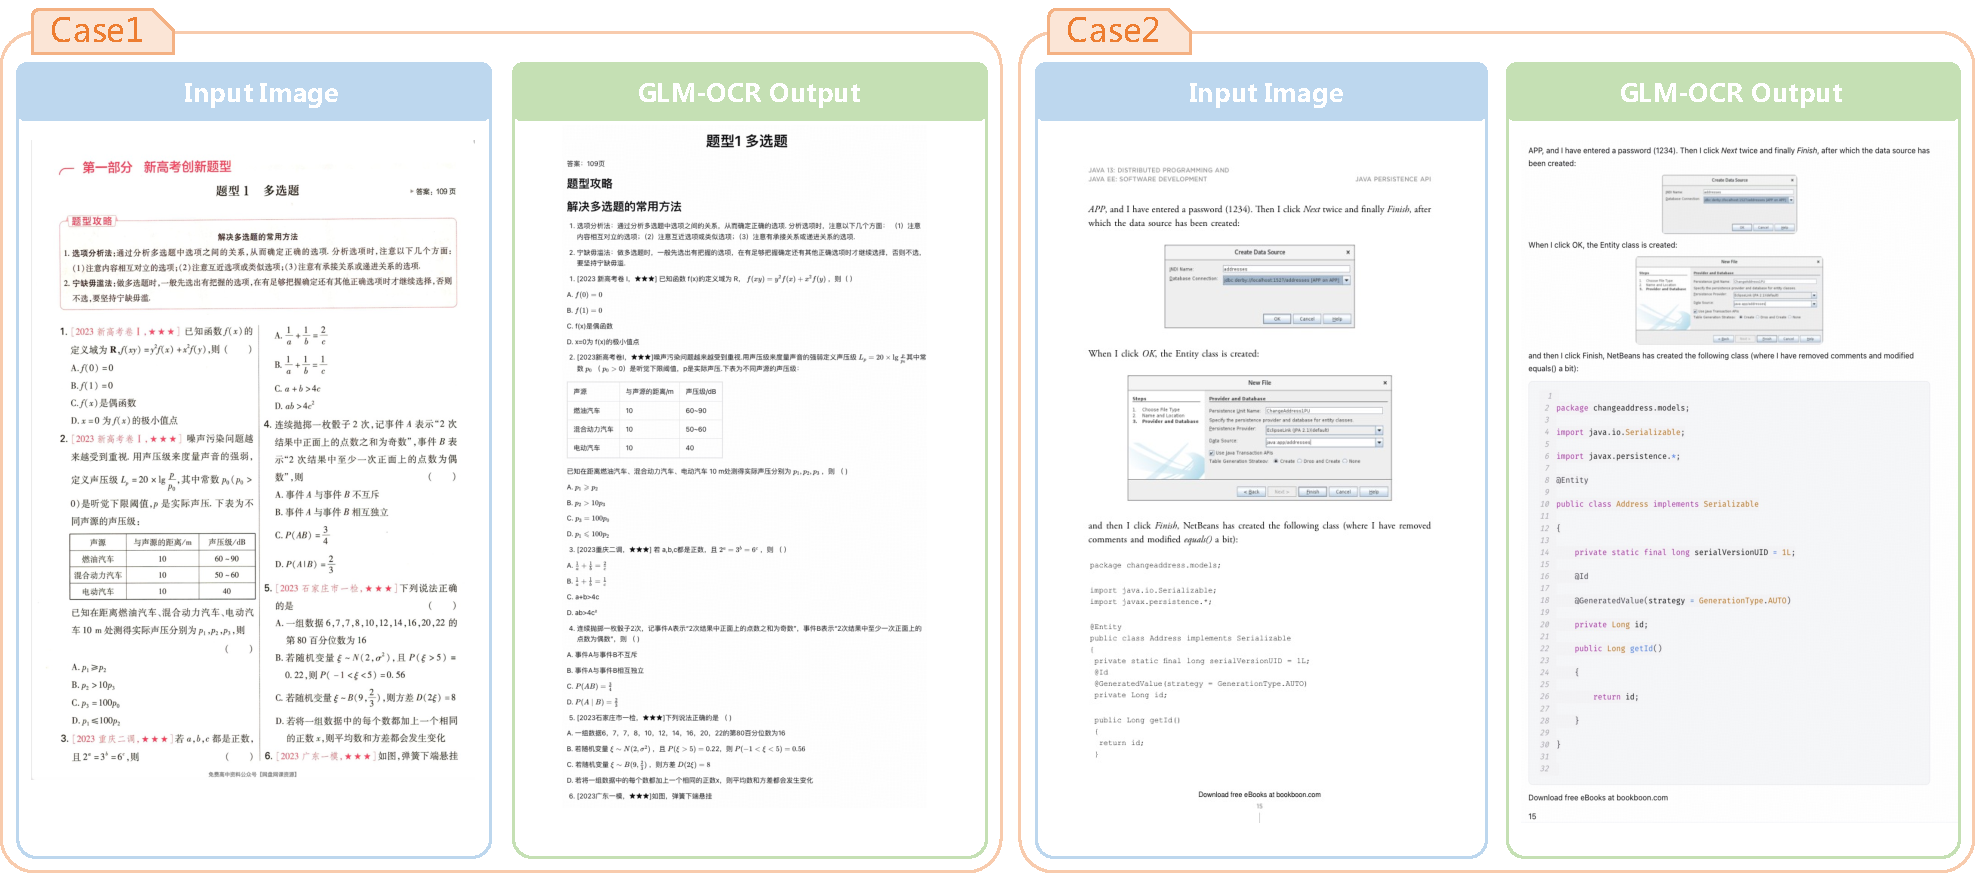
\includegraphics[width=\linewidth]{assets/use_case_sdk.pdf}
\caption{Example of GLM-OCR SDK for complex document parsing.}
\label{fig:use_case_sdk}
\end{figure}

The output is generated in a structured markdown format, preserving logical document hierarchy and structural relationships. The example demonstrates that the SDK supports end-to-end parsing of heterogeneous documents while maintaining structural fidelity and semantic coherence.

\subsection{Lightweight OCR and Information Extraction with the Base Model}

In addition to the SDK, GLM-OCR can be directly used as a standalone model for lightweight OCR and targeted extraction tasks. This mode is appropriate for scenarios requiring lower integration overhead, flexible prompting, or rapid prototyping.

All tasks in this mode are controlled via explicit prompt instructions. Below we describe four primary task categories.

\subsubsection{Text Recognition}

\textbf{Prompt:}
\begin{verbatim}
Text Recognition:
\end{verbatim}

This mode is used for general printed or handwritten text transcription. The model outputs plain text corresponding to the visible textual content in the input image.

\paragraph{Example Scenario.}

\begin{figure}[!h]
\centering
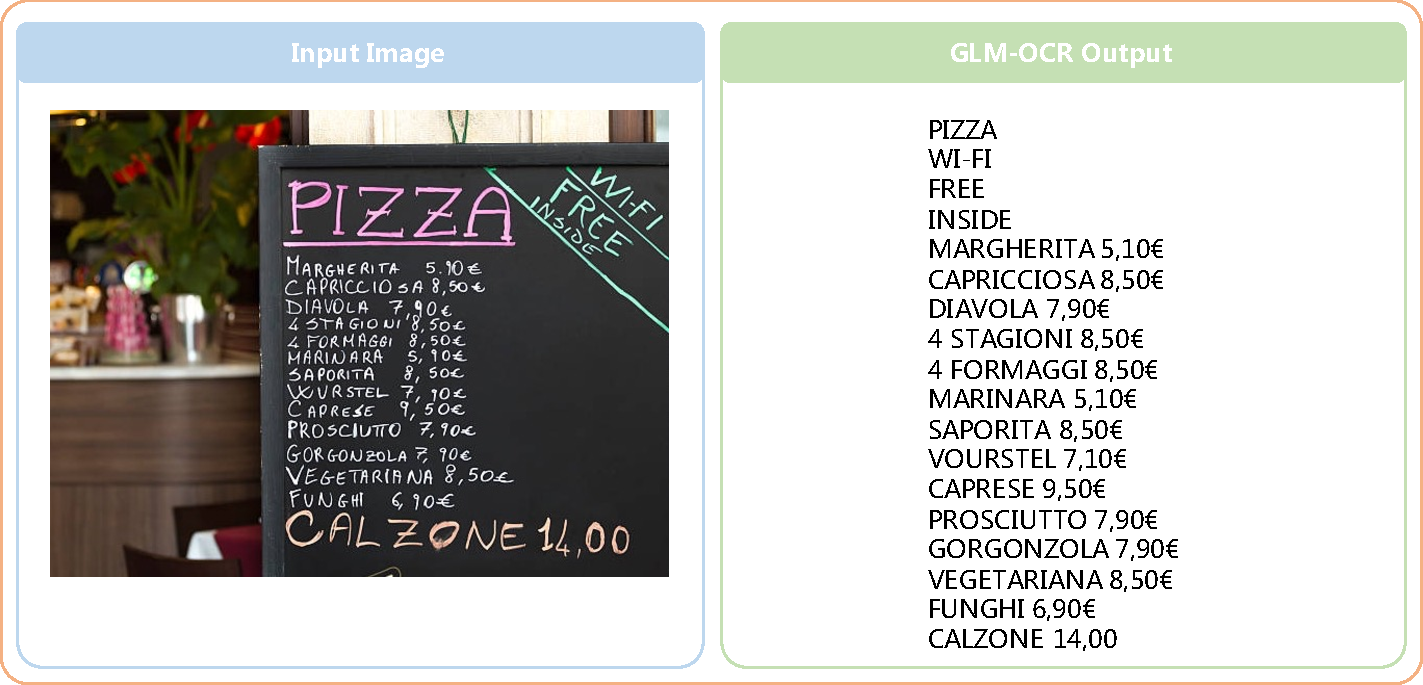
\includegraphics[width=\linewidth]{assets/use_case_text.pdf}
\caption{Example of GLM-OCR Text Recognition.}
\label{fig:use_case_text}
\end{figure}

Figure~\ref{fig:use_case_text} illustrates a real-world text recognition scenario using a restaurant menu board containing multilingual content (e.g., Italian dish names and English phrases) and price annotations with special characters (e.g., the euro symbol). The input image exhibits typical challenges such as handwritten-style fonts, varying character sizes, non-uniform spacing, perspective distortion, and background clutter.

Despite these complexities, the model accurately transcribes the textual content while preserving the original line structure and semantic grouping. In particular, it correctly reconstructs line breaks, capitalization, punctuation, numerical values, and currency symbols (e.g., “5,10€”, “14,00”), demonstrating robustness to layout variations and moderate visual noise. This example highlights the model’s ability to perform reliable optical character recognition in unconstrained, real-world environments.

\subsubsection{Table Recognition}

\textbf{Prompt:}
\begin{verbatim}
Table Recognition:
\end{verbatim}

This task focuses on recovering the structural representation of tabular data. The output may be formatted as Markdown tables or structured text that preserves row and column alignment.

\paragraph{Example Scenario.}

\begin{figure}[!h]
\centering
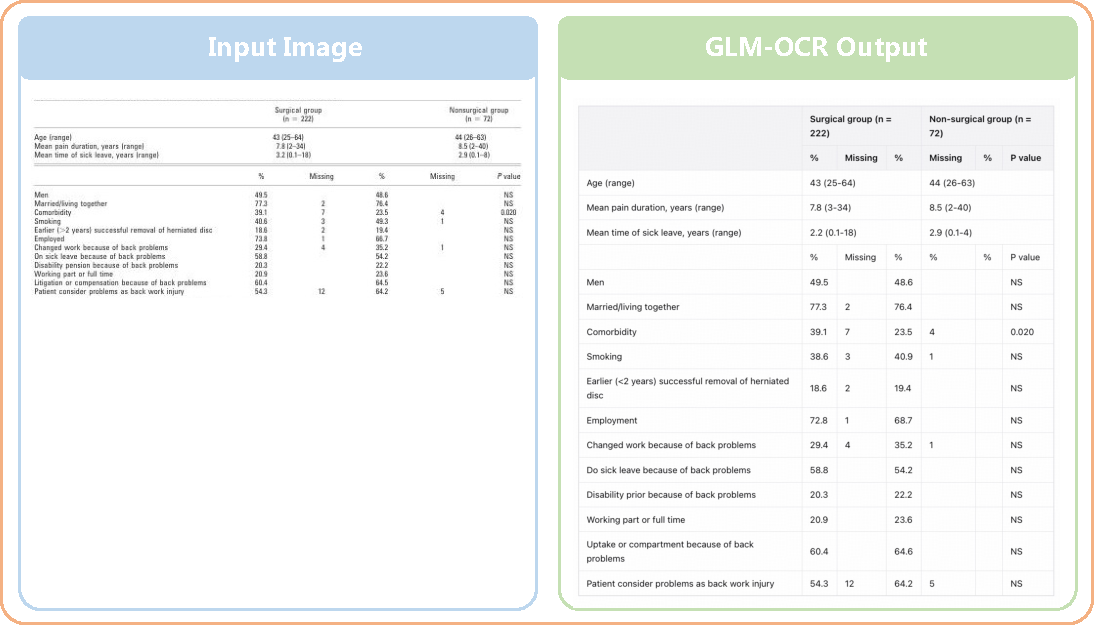
\includegraphics[width=\linewidth]{assets/use_case_table.pdf}
\caption{Example of GLM-OCR Table Recognition.}
\label{fig:use_case_table}
\end{figure}

Figure~\ref{fig:use_case_table} presents a clinical summary table containing hierarchical column headers, merged cells, percentage values, missing-value indicators, and statistical annotations (e.g., p-values). The input image exhibits typical document-analysis challenges, including low contrast, dense numerical content, multi-level header grouping, and complex row–column alignment.

GLM-OCR accurately reconstructs the logical table structure by identifying column groups (e.g., surgical vs.\ non-surgical cohorts), preserving header hierarchies, and correctly aligning numerical entries with their corresponding attributes. In addition to faithfully transcribing cell content, the model maintains structural consistency such as row ordering, column correspondence, and percentage–value pairing. This structured reconstruction enables direct conversion into machine-readable formats (e.g., CSV or spreadsheet tables), thereby facilitating downstream statistical analysis, data validation, and automated reporting workflows.

\subsubsection{Formula Recognition}

\textbf{Prompt:}
\begin{verbatim}
Formula Recognition:
\end{verbatim}

This mode is intended for recognizing mathematical expressions and converting them into structured formats (e.g., LaTeX).

\paragraph{Example Scenario.}

\begin{figure}[!h]
\centering
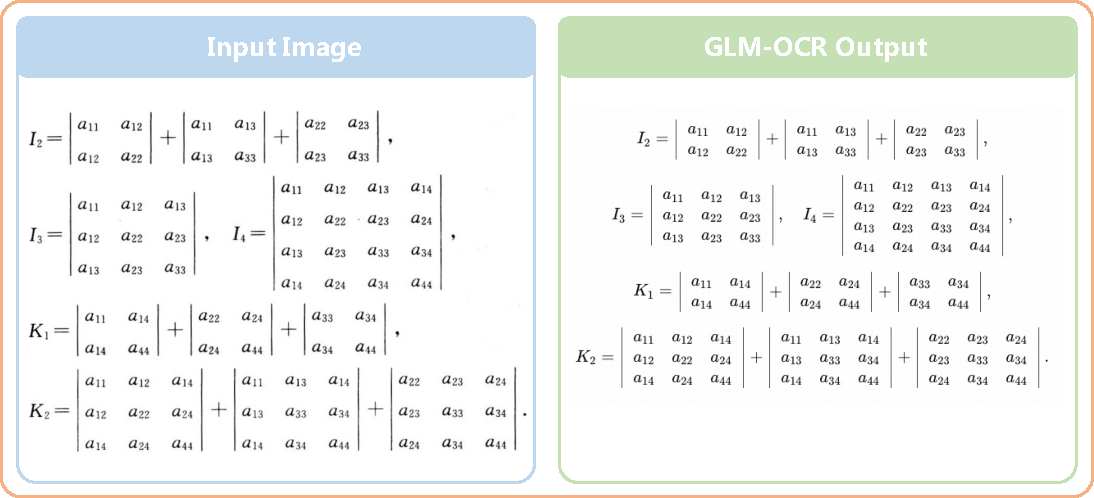
\includegraphics[width=\linewidth]{assets/use_case_formula.pdf}
\caption{Example of GLM-OCR Formula Recognition.}
\label{fig:use_case_formula}
\end{figure}

Given an image containing inline and display equations from a scientific manuscript, the model transcribes the formulas into syntactically valid LaTeX expressions. The output preserves operators, superscripts, subscripts, and fraction structures, enabling direct reuse in academic or technical documentation.

As depicted in Figure \ref{fig:use_case_formula}, given an image containing dense mathematical equations, GLM-OCR accurately transcribes the visual content into syntactically valid LaTeX expressions. The model demonstrates high fidelity in parsing complex two-dimensional spatial layouts, successfully preserving intricate structural elements such as matrices, determinants, and multi-level subscripts. This precise reconstruction eliminates the need for manual correction, enabling direct and seamless reuse in academic and technical documentation.

\subsubsection{Key Information Extraction}

For structured information extraction tasks, the prompt must explicitly specify a strict JSON schema. The model is expected to generate output that conforms to the provided format.

% \textbf{Prompt:}

% \begin{verbatim}
% 请按下列JSON格式输出图中信息:
% {
%     "id_number": "",
%     "last_name": "",
%     "first_name": "",
%     "date_of_birth": "",
%     "address": {
%         "street": "",
%         "city": "",
%         "state": "",
%         "zip_code": ""
%     },
%     "dates": {
%         "issue_date": "",
%         "expiration_date": ""
%     },
%     "sex": ""
% }
% \end{verbatim}

\paragraph{Example Scenario.}

\begin{figure}[!h]
\centering
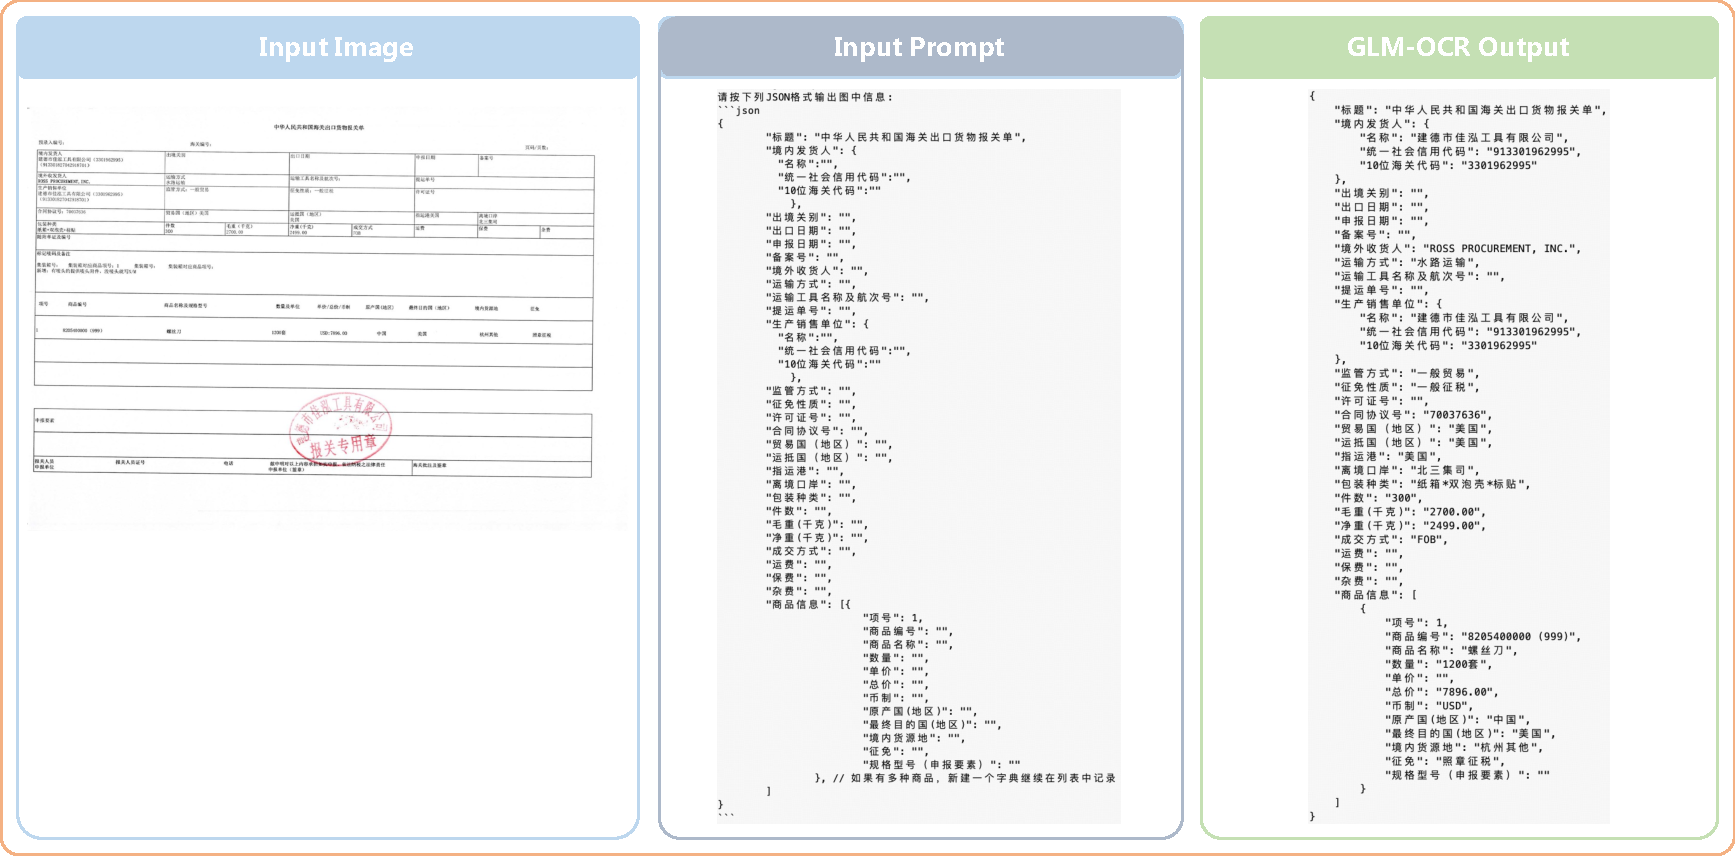
\includegraphics[width=\linewidth]{assets/use_case_kie.pdf}
\caption{Example of GLM-OCR Key Information Extraction.}
\label{fig:use_case_kie}
\end{figure}

In a representative example involving a dense customs declaration form, the model successfully extracts structured fields based on a detailed input prompt. It accurately populates complex, nested JSON entities—such as shipper details, unified social credit codes, and itemized goods information—directly from the visual layout. The output strictly adheres to the user-provided JSON schema, eliminating hallucinated keys and facilitating seamless integration into automated processing pipelines or structured databases.

\subsection{Summary of Usage Paradigms}

The two usage modes address complementary needs:

\begin{itemize}
    \item \textbf{GLM-OCR SDK} is designed for comprehensive, layout-aware, multi-element document parsing in production environments.
    \item \textbf{Base model prompting} enables lightweight, flexible OCR and targeted information extraction for modular or task-specific applications.
\end{itemize}

Together, these paradigms allow GLM-OCR to support a broad spectrum of document understanding workflows, ranging from rapid prototyping to enterprise-scale deployment.